\documentclass{standalone}
\usepackage{tikz}

\begin{document}

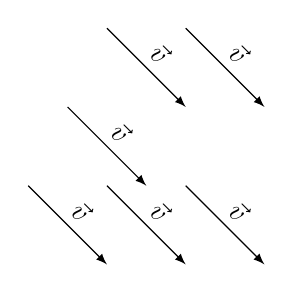
\begin{tikzpicture}
  \foreach \x/\y in {0/0,1/0,2/0,0.5/1,1/2,2/2} {
    \draw[-latex] (\x,\y) -- ++(1,-1) node[midway,above,sloped] {$\vec v$};
  }
\end{tikzpicture}

\end{document}